\section{Kubernetes. ReplicaSet. Deployment. Recreate. Rolling Update. StatefulSet. StatefulSet:
headless Service. DaemonSet. Job.}

\begin{figure}[H]
	\centering
	\begin{minipage}[b]{0.4\textwidth}
		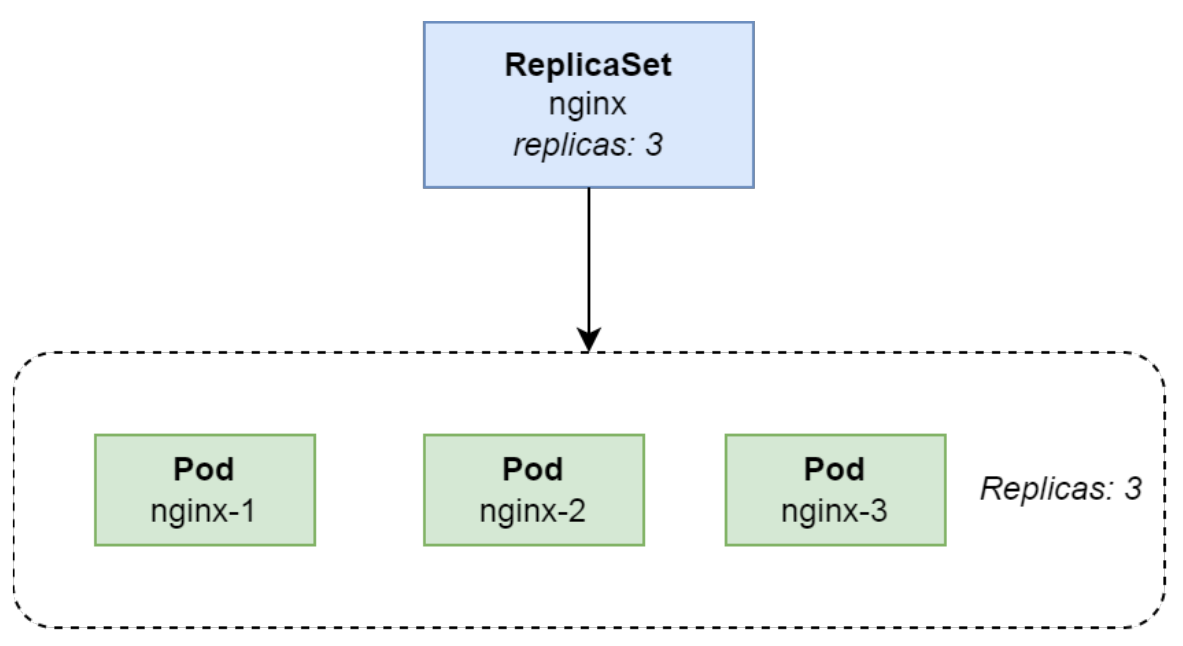
\includegraphics[width=\textwidth]{images/rset.png}
        \caption{Replica Set scheme}
	\end{minipage}
\end{figure}

Позволяет поднимать по несколько подов, автоматически рестартит поды
при падении.

Deploy происходит постепенно на всех подах и репликах.

\begin{figure}[H]
	\centering
	\begin{minipage}[b]{0.4\textwidth}
		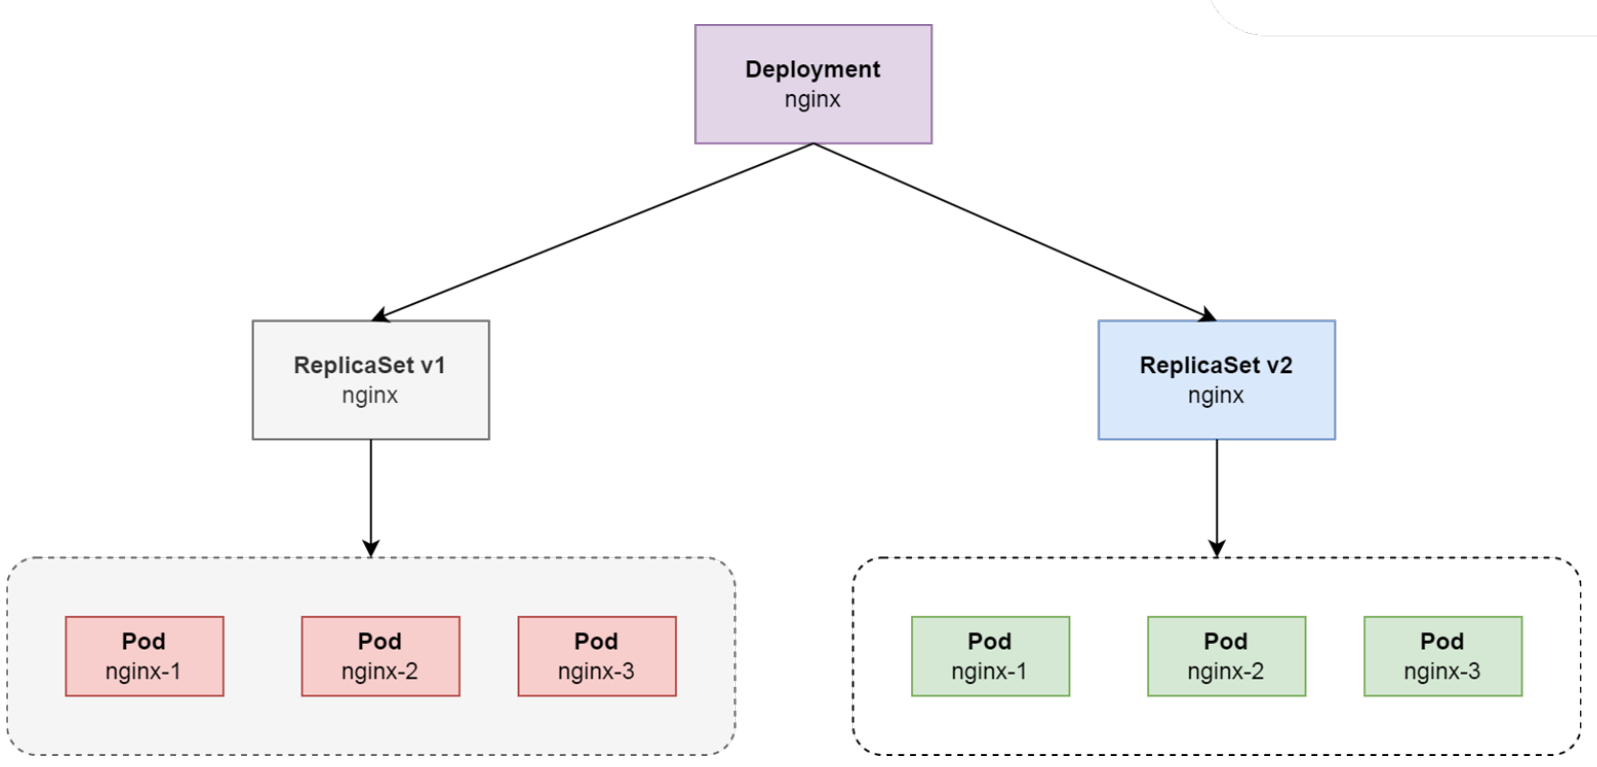
\includegraphics[width=\textwidth]{images/kdep.png}
        \caption{Deploy scheme}
	\end{minipage}
\end{figure}

Стратегии обновления:
\begin{itemize}
    \item Recreate
    
    Все старые поды удаляются и создаются новые.
    \item Rolling Update
    
    По парам создаются новые поды и удаляются старые.
\end{itemize}

\subsection*{Best practices}

StatefulSet - паттерн организации подов:
\begin{itemize}
    \item Также основан на репликах
    \item Однако каждая реплика использует свой PVC
    \item PVCs могут быть созданы заранее или динамически
    \item Переживут воссоздание реплик, но могут ограничить планирование подов только узлами, на которых есть экземпляры PVC
    \item В итоге: сохраняем состояние. Идеально для баз данных
\end{itemize}

StatefulSet headless service: headless создает DNS записи для всех реплик
StatefulSet. Можно получить доступ к нужной реплике по имени хоста.

\D{
    DaemonSet - совокупность узлов, на каждый из которых установлен под
    с определенной версией функционала.
}

\begin{figure}[H]
	\centering
	\begin{minipage}[b]{0.6\textwidth}
		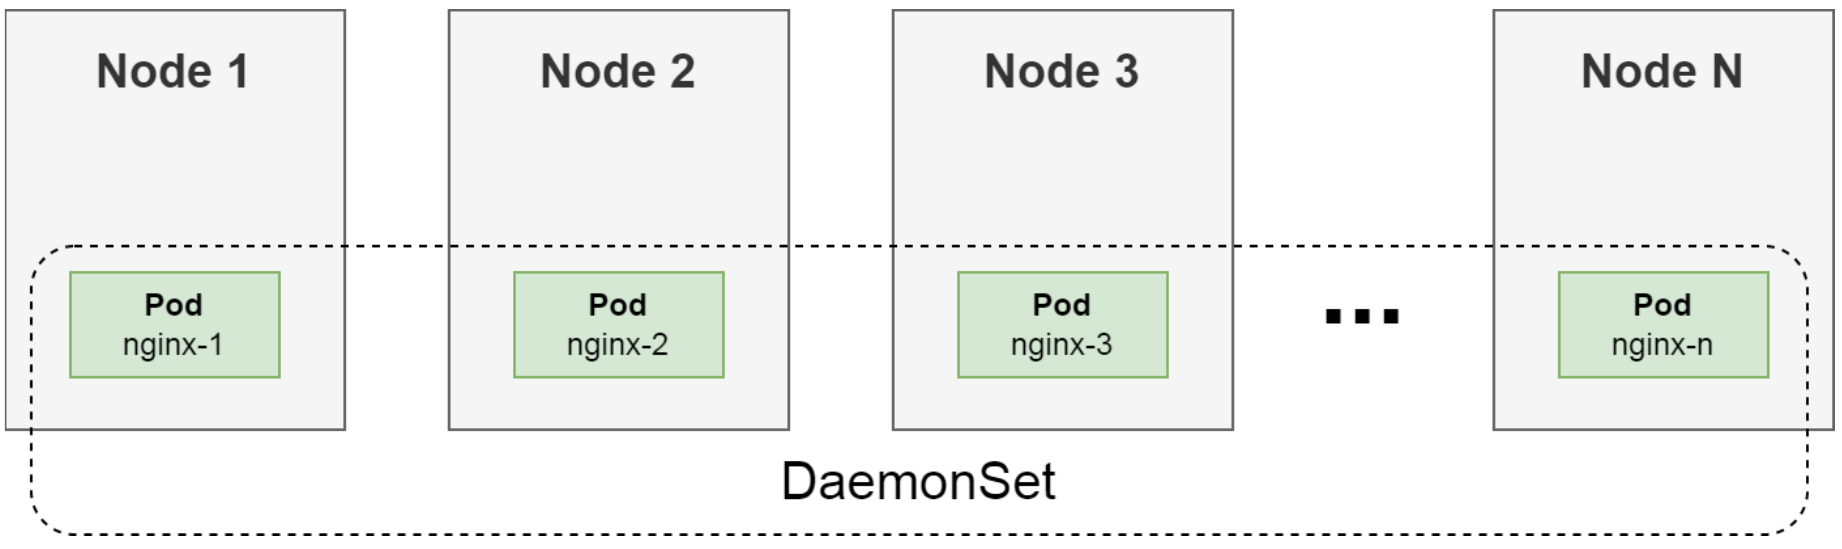
\includegraphics[width=\textwidth]{images/kds.png}
        \caption{DaemonSet}
	\end{minipage}
\end{figure}

\D{
    Job - сценарий исполнения кода на всех задействованных подах.

    Может понадобиться для сбора логов / резервного копирования.
}